\subsection{28 августа. Д.р. Чиринкол}

\textit{Метеоусловия: утром, днём, вечером переменная облачность, кратковременные дожди}

\begin{figure}[h!]
	\centering
	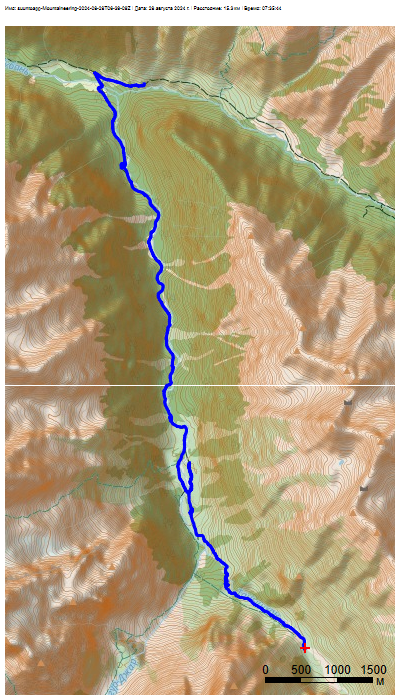
\includegraphics[angle=0, width=0.7\linewidth]{../pics/mini_maps/28}
	\label{fig:mini_28}
\end{figure}

*воспоминания вики: проснулись, пошли по кустарникам вдоль реки, вышли к мужикам, гоняющим коровок, вдоль накатанной дороги и по цивильным мостам дошли до места стоянки*

\clearpage